\documentclass[11 pt]{article}
\usepackage[margin=1in]{geometry}
\usepackage{setspace}
\usepackage{tabularx}
\usepackage{sectsty}
\usepackage{cite}
\usepackage{graphicx}
\usepackage[labelsep=space]{caption}

\captionsetup{labelfont=bf}
\renewcommand{\thefigure}{\arabic{figure}.}
\renewcommand{\rmdefault}{phv} % Arial
\renewcommand{\sfdefault}{phv} % Arial
\sectionfont{\normalsize}
\subsectionfont{\normalsize}
\renewcommand\thesection{\Alph{section}.}
\renewcommand\thesubsection{\Alph{section}.\arabic{subsection}}
\begin{document}
{\large \centerline{\emph{Habronattus clypeatus} Temperature Trial Male Signal Processing/Analysis Protocol}}
\section{Materials}
\subsection{Materials}
\begin{itemize}
\item{video files}
\item{tally counter}
\item "animal\_info.csv" file containing information for each trial and individual (see figure \ref{aninfo} )
\end{itemize}
\subsection{Software}
\begin{itemize}
\item{ffmpeg (version 2.1.3)}
\item{audacity(version 2.0.5)}
\item {text editor}
\item custom python scripts (python version 2.7):
\begin{itemize}
\item maleviban.py: contains functions for analysis; not called directly
\item overall\_analysis.py: actually does the analysis for every individual, makes one .csv file for each individual
\item all\_inds.py: compiles all information from each individual into one .csv file
\item config.py: configuration file that allows shared variables between other scripts.  Need to have this file in the same directory as the others.
\end{itemize}
\item python modules:
\begin{itemize}
\item numpy
\item scipy
\item matplotlib
\item pypeaks
\item tkMessageBox
\end{itemize}
\item Custom R Scripts (version 3.1.0)
\begin{itemize}
\item plots.r: used to make simple (Tukey) plots of all features
\item q10\_stuff.R: used for regression analysis of all features
\end{itemize}
\item DO\_EVERYTHING.sh: bash script to execute all necessary code to do data processing/analysis
\end{itemize}


\section{Wav Annotation Methods}
\subsection{Converting Videos to .wav Files}
\subsection{Extracting Data from .wav Files}
\begin{enumerate}
\item{Open .wav file in audacity.}
\item{Use the zoom functions to make the .wav file fill about 3/4 of the screen.}
\end{enumerate}
\subsection{Scrape, Thump and Buzz Durations}
\begin{enumerate}
\subsection {Thumps}
\item Locate the first thump in the recording that is followed by scrapes.  In most recordings, this will be the last thump of the intro display (a series of 6 or so thumps).
\item{Highlight and label the thump as shown in Figure \ref{thumpdur}.  Start the highlight where the trace begins to dip down before the main thump.  End the highlight when the oscillations of the trace after the thump attain a steady amplitude. Label the thump "t1".}
\item{Press ctrl+b to bring up labeling window. (or change the keyboard shortcut.  I prefer "b" instead of "ctrl + b"}
\item Locate and label every subsequent thump (t2, t3, etc.).  If you are using the viban python functions, the number you use doesn't matter, because they are listed in the order that they occur in the recording.

\subsection {Buzzes}
\item Highlight and label  each buzz as indicated in Figure \ref{buzzdur}. Begin the highlight when the amplitude first begins to increase.  End the highlight when the buzz comes to an abrupt end. Label the buzz "b1".
\subsection {Scrape Rates}
\item {Start at t1, and highlight the area that contains scrapes between t1 and t2. Label this region "r1\_" Do this for every section of consecutive scrapes that contains 5 or more legible scrapes.  Leave out any areas where scrapes are difficult to discern.  See Figure \ref{srate}}
\item After you have labeled all scrape regions, go back to the "r\_1.  Using the mechanical tally counter or another method, count every scrape in the region.  Put this number into the label after the underscore, eg: "r1\_105".  These numbers will be stripped out to calculate scrape rates later.
\subsection{Scrapes}
\item Highlight and label a total of 20 scrapes, spread more or less evenly throughout the recording (but each one within a rate region that you defined above.  See Figure \ref{scrapedur}.
\end{enumerate}
\section{Generating Duration, Rate, and Frequency Data}
\subsection{A Few Notes About Setting Up your Data}
\begin{itemize}
\item First, your folder organization is important.  The analysis python scripts are set up to specifically look for folders in a certain configuration.  You should have a "data" folder.  Inside this folder should contain one folder for each individual (not each trial), named for each individual.
\item Inside the folder for each individual, should be one folder for each trial.  These folders should be named "individualname\_trialnumber" (eg: 5-41).  For my purposes, I made each trial number the number on the video, instead of some indication of the treatment (to avoid biasing data analysis).
\item Inside each "trial" folder, you must have an annotation file (eg: "5-41.labels.txt").
\item An "animal\_info.csv" file must exist somewhere, but you get to pick directly where to pull it from.  It makes most sense to put it in the top-level "data" folder.  
\item .wav files are organized slightly differently.  There needs to be a "data" folder containing a folder named for each individual as above.  However, do not make separate folders for each treatment.  Simply place all .wav files associated with an individual in that individual's folder.
\end{itemize}
\subsection{Running python scripts}
This is fairly straightforward.  At the end of the process, you will have: csv files for each individual containing duration data for each annotated feature, and peak frequency data for each buzz.
\begin{enumerate}
\item Run the {\bfseries overall\_analysis.py} script.
\item Troubleshooting overall\_analysis.py  
\begin{itemize}
\item The  most common issue is a misnamed or incorrectly-placed file.  Check to make sure your files are properly named and in the right folder.
\item Another issue may be if your "animal\_info.csv" file is in a strange format.  Check that file.
\item The frequency analysis portion of this is in beta mode.  In its current foundation, the frequency-finding function is wonky for very low-amplitude signals, and will give a teeny tiny amplitude and a large frequency.  For the moment, you will need to look for these in the "duration\_data" files, then use the test.py function to individually pull up problematic buzzes. Choose the "show spectral data graphs" and get the true peak data, hand-inputting the data into the duration\_data file.
\end{itemize}
\item Run the {\bfseries all\_inds.py} script.
\item Troubleshooting all\_inds.py.
\begin{itemize}
\item Since this script doesn't involve any calculation, and only refers to files that were generated by overall\_analysis.py, there shouldn't be too many problems.  
\end{itemize}
\end{enumerate}

\begin{figure}[htp]
\centering
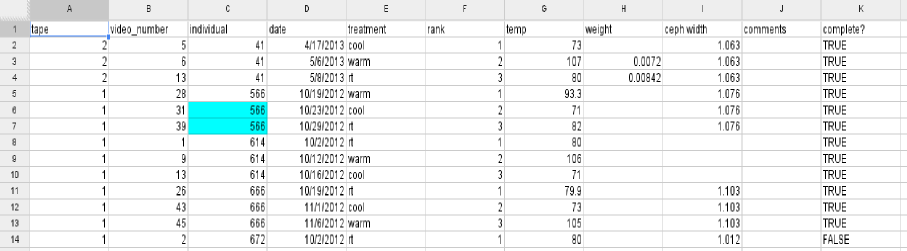
\includegraphics[scale=.85]{animal_info.png}
\caption{Example of the animal information data file.  Fields described below.  {\bfseries tape:} the video tape number used, {\bfseries video number:} number of video on the tape, {\bfseries individual:} individual number,  {\bfseries date:} date of recording, {\bfseries rank:} order of this trial for this individual (1 being first, 3 being last), {\bfseries temp:} temperature of trial (in Farenheit), {\bfseries weight:} weight of spider (measured after each trial), {\bfseries ceph width:} width of cephalothorax of each individual (measured once), {\bfseries comments:} any comments on analysis (no commas can be used in this field), {\bfseries complete?:} whether this individual has a complete set of data associated with it (for repeated-measures, as opposed to simple regression-based, analysis)}
\label{aninfo}
\end{figure}

\begin{figure}[htp]
\centering
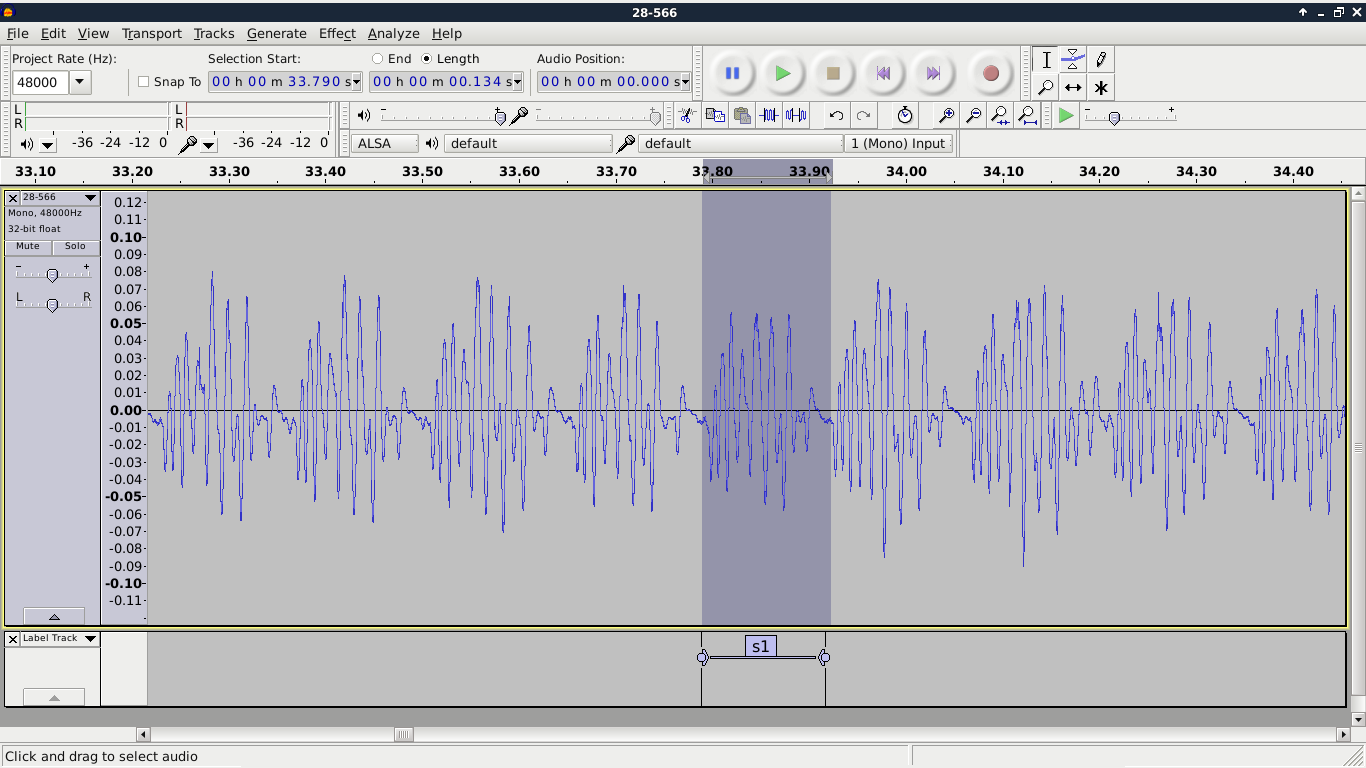
\includegraphics[scale=.30]{scrape_duration.png}
\caption{Screenshot showing how to measure the duration of a scrape.  Note the label "s1" at the bottom.}
\label{scrapedur}
\end{figure}

\begin{figure}[htp]
\centering
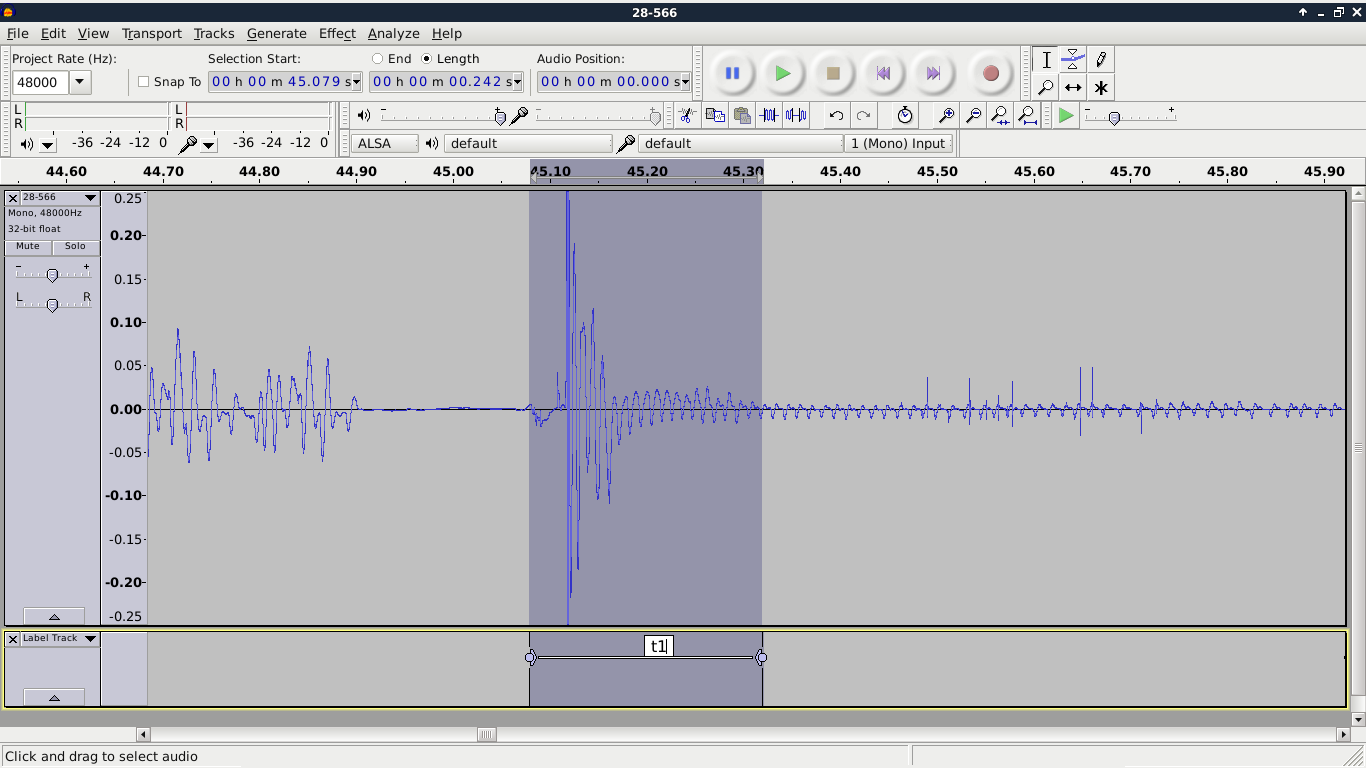
\includegraphics[scale=0.30]{thump_duration.png}
\caption{Screenshot showing how to measure the duration of a thump.  Note the label "t1" at the bottom.}
\label{thumpdur}
\end{figure}

\begin{figure}[htp]
\centering
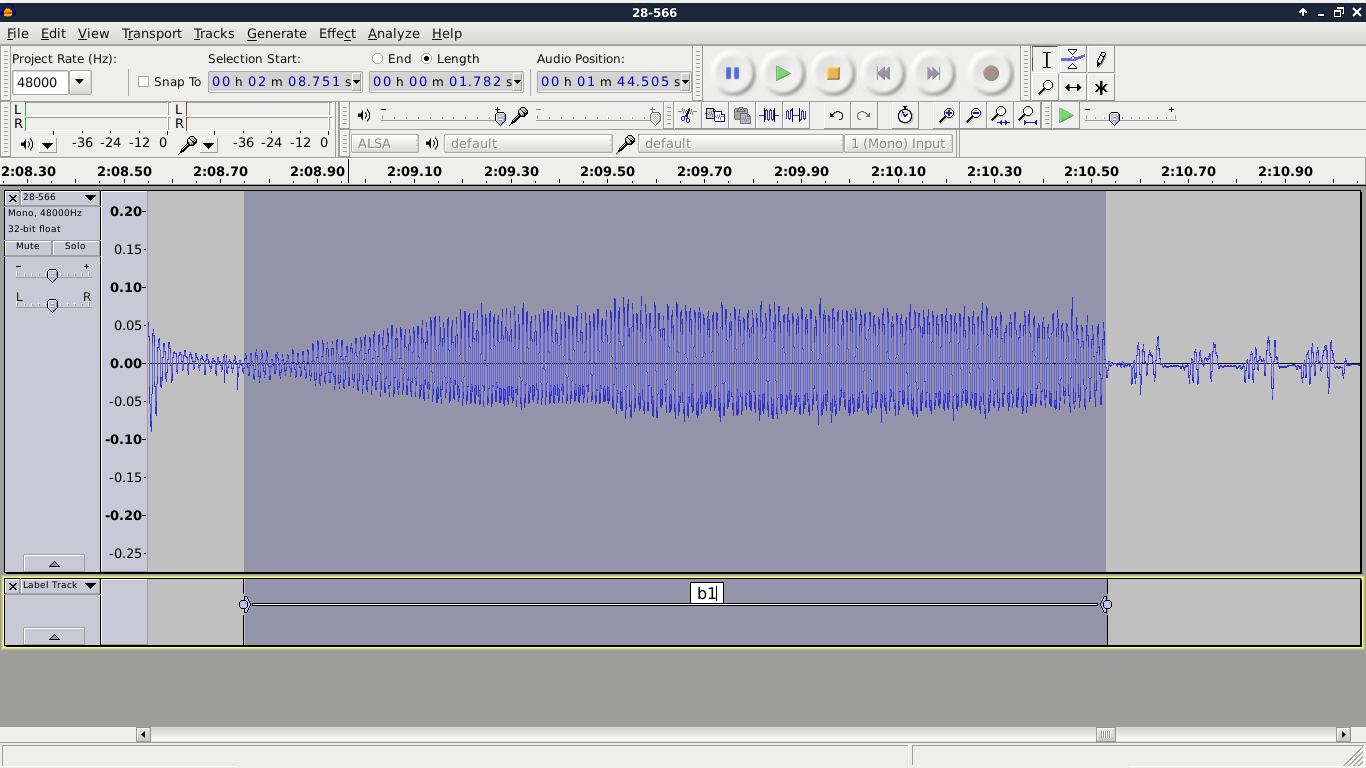
\includegraphics[scale=0.30]{buzz_duration.png}
\caption{Screenshot showing how to measure the duration of a thump.  Note the label "b1" at the bottom.}
\label{buzzdur}
\end{figure}

\begin{figure}[htp]
\centering
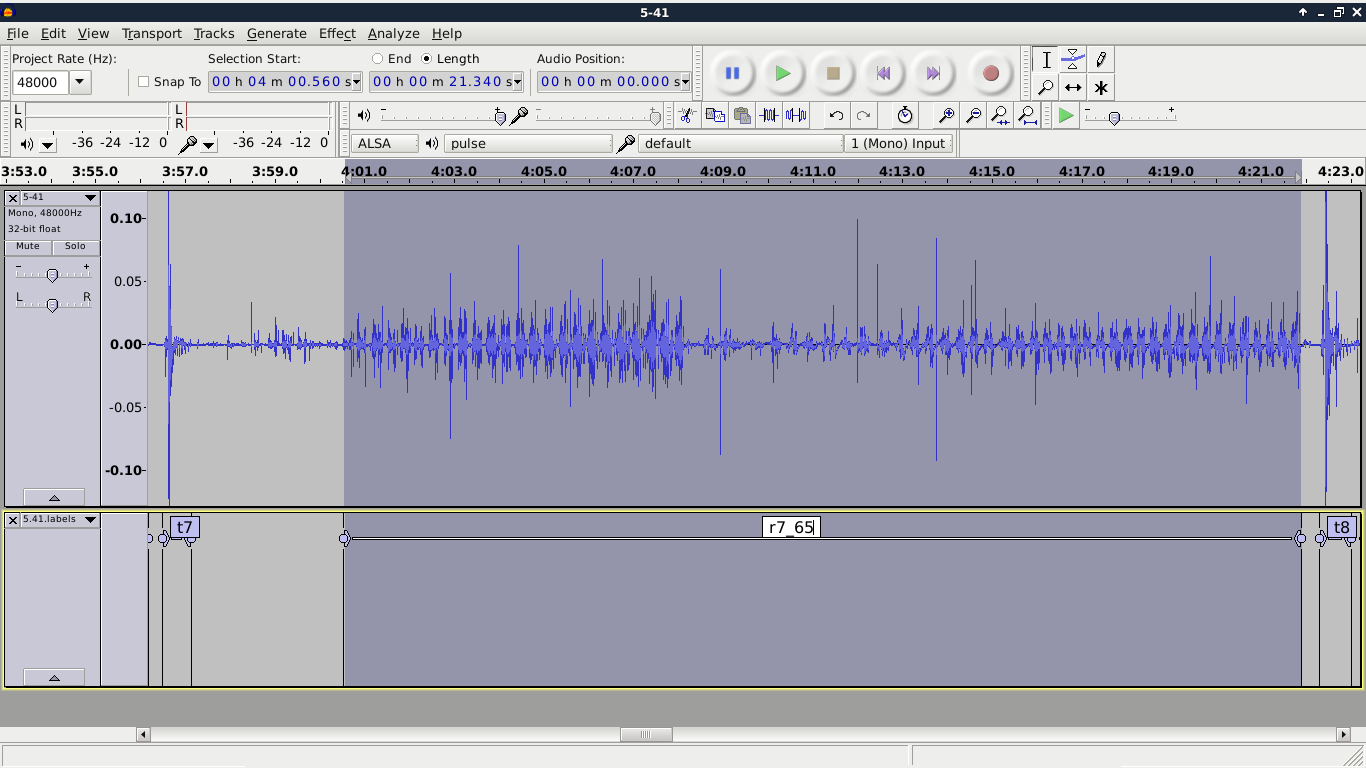
\includegraphics[scale=0.30]{scrape_rate.png}
\caption{Screenshot showing how to measure scrape rate.  Note the thumps on either side of the scrape region. You must count each individual scrape and input the number after the "\_". Also note that regions that are unclear were left out.}
\label{srate}
\end{figure}
\end{document}